\subsection{Systementwurf und -analyse}
Systementwurf: Hier mein angepasstes Architekturmodell -> konkretes Architekturmodell mit Sensoren, Edge Device (RPI), SCP (CF) mit Leo IoT Services; AWS SNS mit API-Schnittstellen
\\Hier irgendwo auch anmerken in Bezug auf 2.3.3 SAP Leonardo und in der Evaluation ausführlicher vllt, dass zwar der Mehrwert in kombinierter Anwendung besteht, man hier aufgrund einer prototypischen Implementierung und es Bezugs auf IoT nur auf ein Leo-Produkt bezogen wird

\subsubsection{Systemarchitektur}

hier generelle Architektur von SAP Leonardo mit SCP

SOA - Service Orientierte Architektur
\begin{figure}[H]
    \centering
    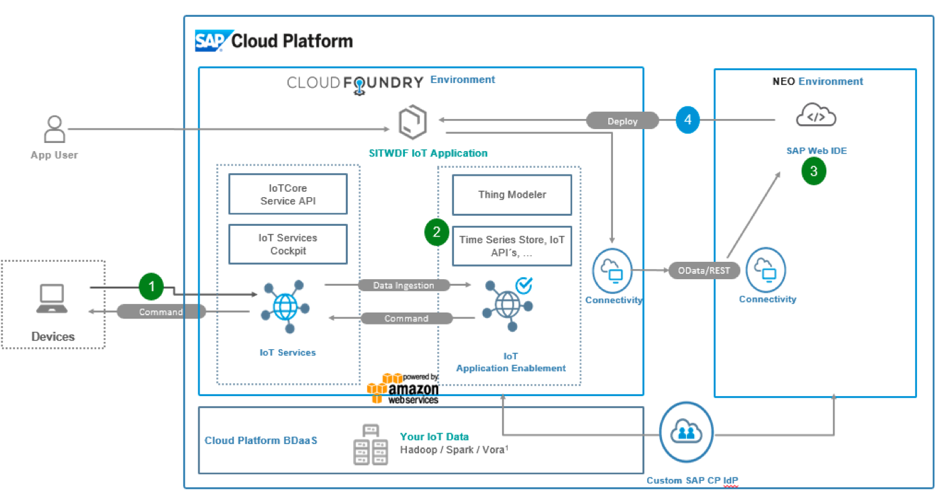
\includegraphics[width=1.0\linewidth]{pictures/sap_architecture}
    \caption[Referenzarchitektur von SAP]{Architektur von SAP \citep{Ganz2019}}
    \label{fig:filename_without_extension}
\end{figure}

\subsubsection{SCP Internet of Things Services}

\begin{figure}[H]
  \centering
  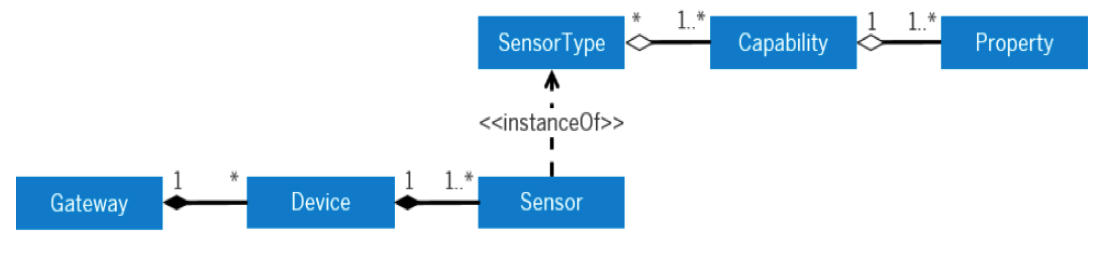
\includegraphics[width=1.0\linewidth]{pictures/device_model}
  \caption[Gerätemodell]{Gerätemodell}
  \label{fig:filename_without_extension}
\end{figure}

\subsubsection{REST API}

\subsubsection{Edge-Processing}

Protokolle der Edge Server CoAP, File, Modbus, MQTT, OPC UA, REST, SigFox, SNMP
\subsubsection{Destinations}
Destinations: Warum braucht man Destinations und welche man benötigt (SNS),  wenn man kommunizieren will mit
Externe Services wie AWS SNS
Interne Kommunikation der SCP CF und NEO
Communication zwischen Cloud Services AWS SNS und SAP Leonardo

\subsubsection{Message Processing}
Leonardo IoT, SQL Kafka: Ich hab Leonardo IoT benutzt (in prototype erwähnen)

\subsubsection{Sicherheit}
OAuth, SSL/TLS, SAML 2.0: erklären, was SAP und AWS auch eventuell haben

\subsubsection{Kompatibiliät mit Referenzarchitektur}

\begin{figure}[H]
  \centering
  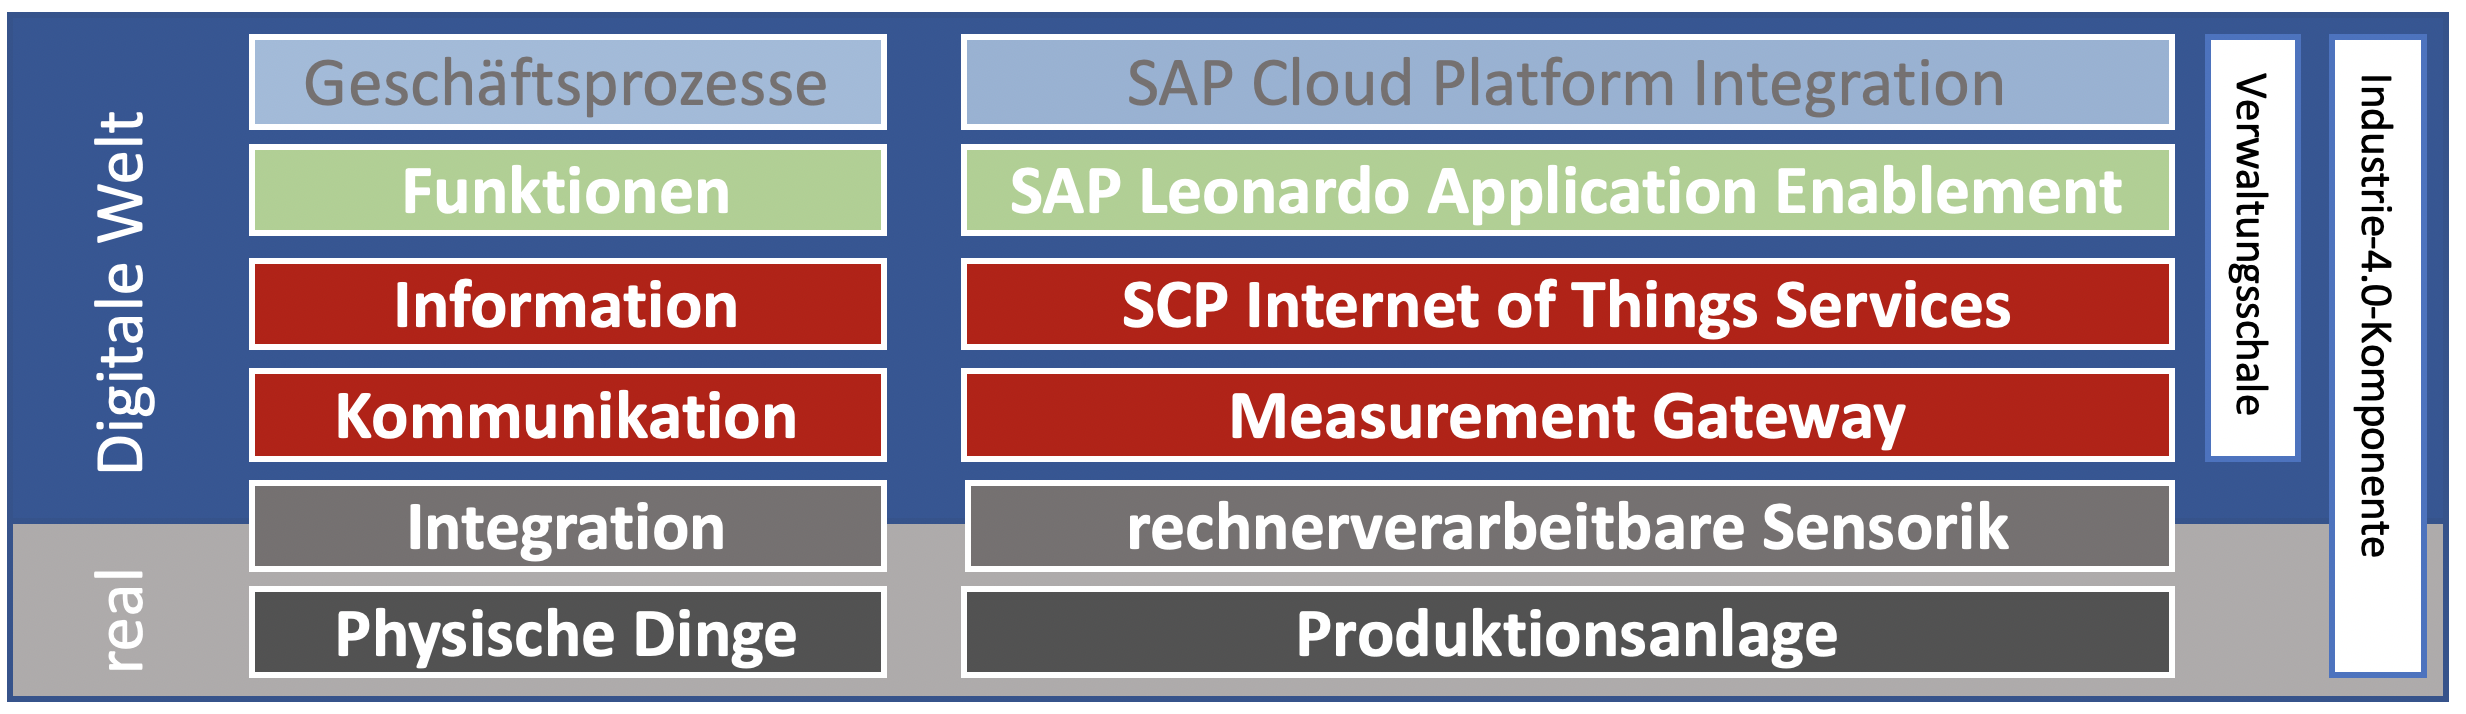
\includegraphics[width=1.0\linewidth]{pictures/rami_custom1}
  \caption[Referenz zu den Schichten der RAMI 4.0]{Referenz zu den Schichten der RAMI 4.0}
  \label{ramicustom}
\end{figure}

\subsubsection{Systementwurf gemäß Architekturkonzept}

eigene Architektur aufmalen

